 \documentclass[a4paper,twocolumn]{article}
 % General document formatting

 \usepackage[parfill]{parskip}
 \usepackage[utf8]{inputenc}
\usepackage{graphicx}

 % Related to math
 \usepackage{amsmath,amssymb,amsfonts,amsthm}
 
 \begin{document}


 	\begin{figure*}
\begin{minipage}{0.45\textwidth}
	With retries:
	\centering
	\scalebox{.5}{
	\includegraphics[trim=0.4cm 0.5cm 0.4cm 0.4cm]{../Fig2a.pdf}
	}
\end{minipage}\hfill
\begin{minipage}{0.45\textwidth}
	Without retries:
	\centering
	\scalebox{.5}{
		\includegraphics{Fig2a.pdf}
	}
\end{minipage}
\caption{Comparison for Fig. 2a}
\end{figure*}



\begin{figure*}
\begin{minipage}{.45\textwidth}
		With retries:
	\centering
	\scalebox{.5}{
		\includegraphics[trim=0.4cm 0.5cm 0.4cm 0.4cm]{../Fig2b.pdf}
	}
\end{minipage}\hfill
\begin{minipage}{.45\textwidth}
	Without retries:
	\centering
	\scalebox{.5}{
		\includegraphics{Fig2b.pdf}
	}
\end{minipage}
\caption{Comparison for Fig. 2b}
\end{figure*}

 	\begin{figure*}
\begin{minipage}{0.45\textwidth}
	With retries:
	\centering
	\scalebox{.4}{
		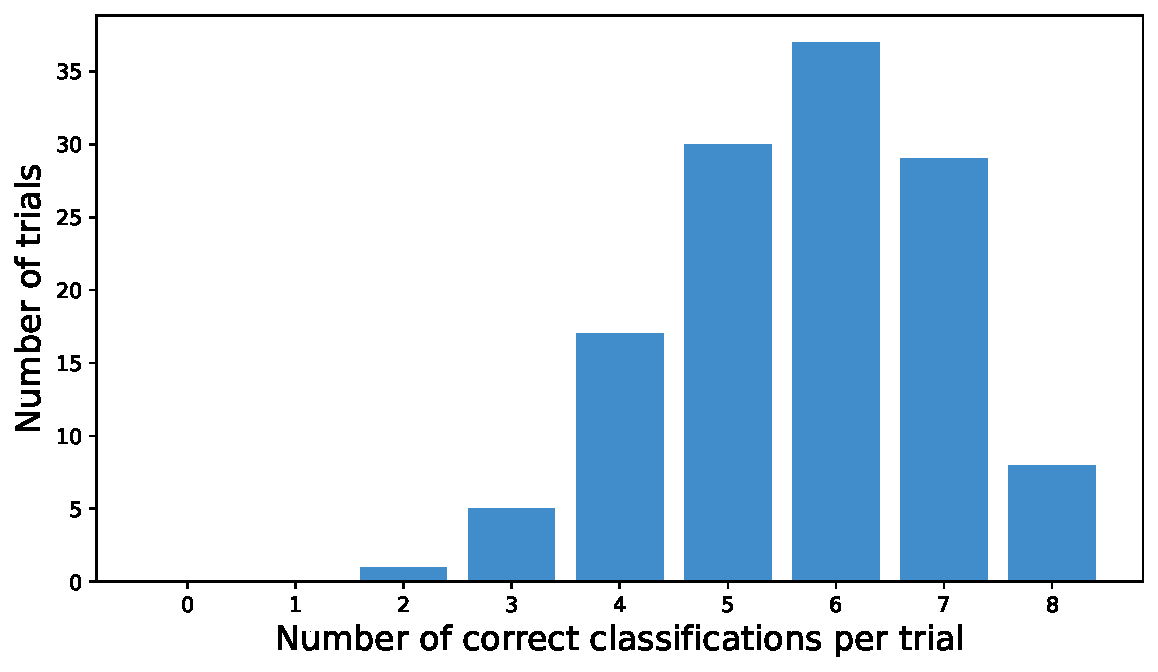
\includegraphics{../Fig3.pdf}
	}
\end{minipage}\hfill
\begin{minipage}{0.45\textwidth}
	Without retries:
	\centering
	\scalebox{.4}{
		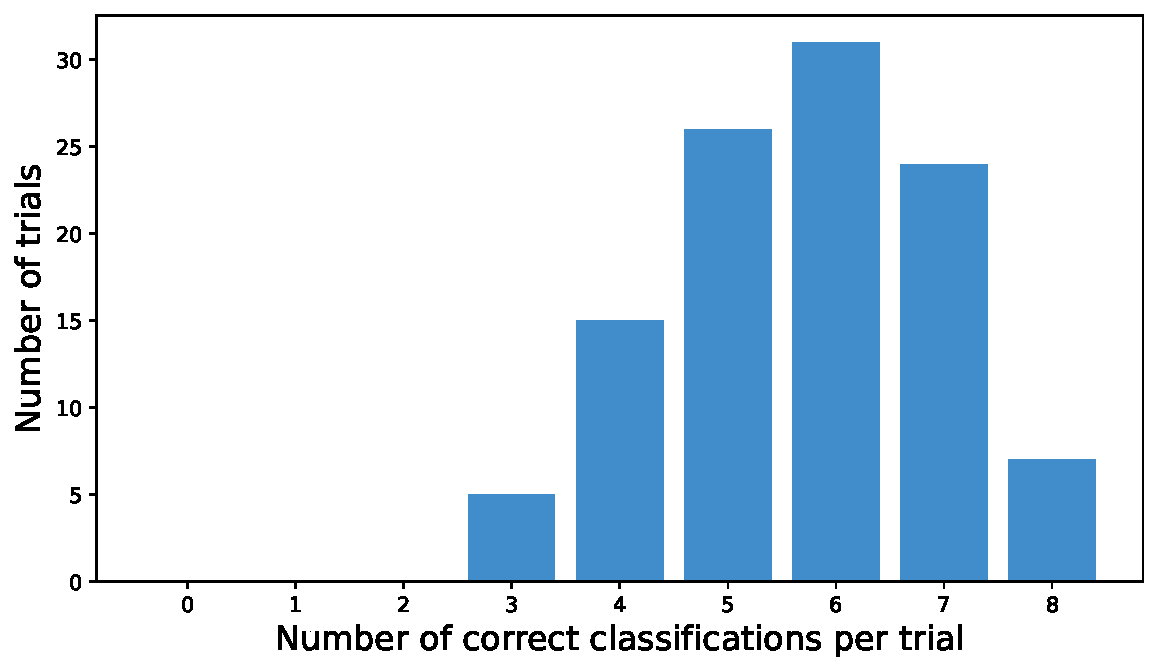
\includegraphics{Fig3.pdf}
	}
\end{minipage}
\caption{Comparison for Fig 3}
\end{figure*}


 	\begin{figure*}
	\begin{minipage}{0.45\textwidth}
		With retries:
		\centering
		\scalebox{.45}{
			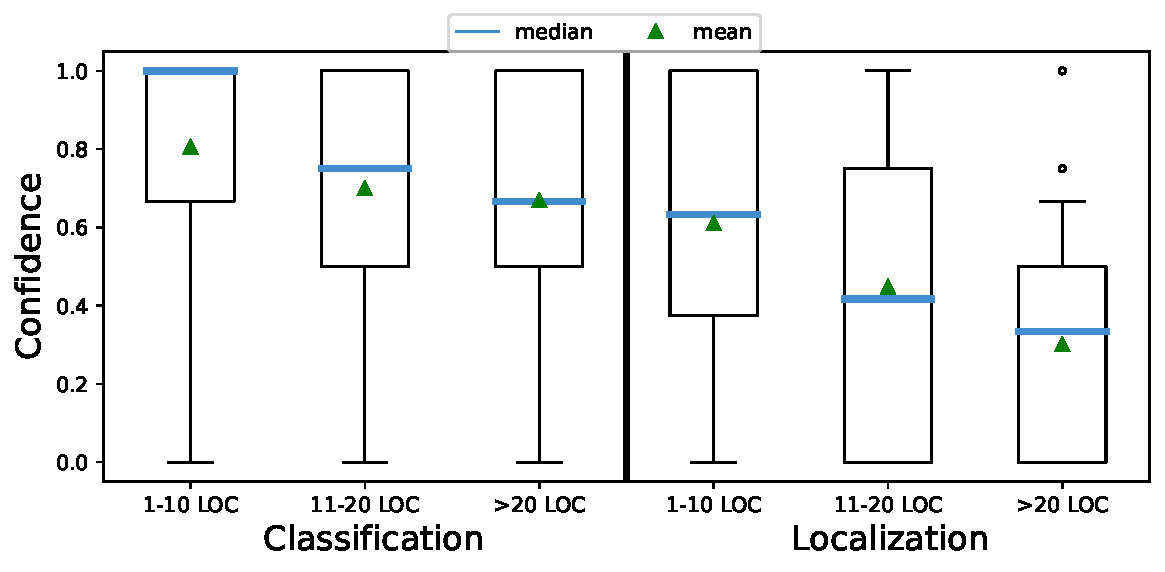
\includegraphics{../Fig4a.pdf}
		}
	\end{minipage}\hfill
	\begin{minipage}{0.45\textwidth}
		Without retries:
		\centering
		\scalebox{.45}{
			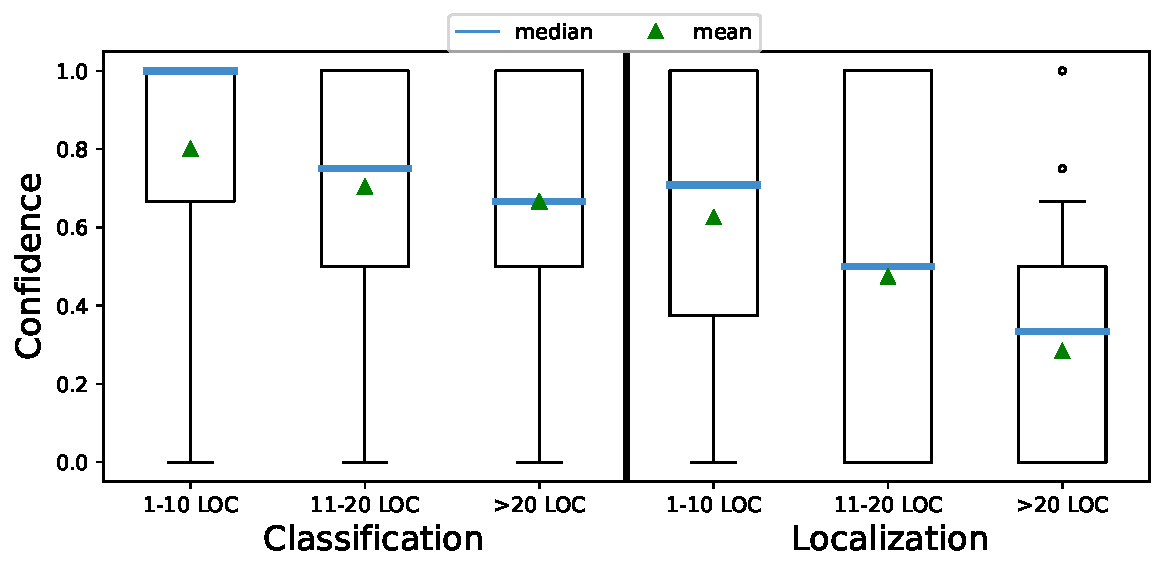
\includegraphics{Fig4a.pdf}
		}
	\end{minipage}
	\caption{Comparison for Fig 4a}
\end{figure*}

 	\begin{figure*}
	\begin{minipage}{0.45\textwidth}
		With retries:
		\centering
		\scalebox{.45}{
			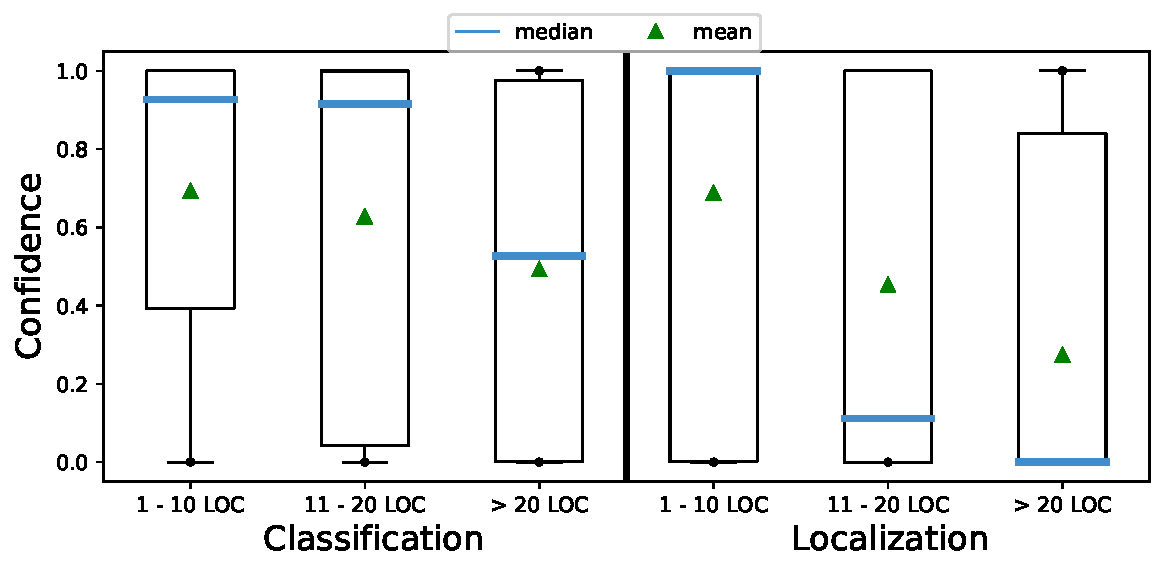
\includegraphics{../Fig4b.pdf}
		}
	\end{minipage}\hfill
	\begin{minipage}{0.45\textwidth}
		Without retries:
		\centering
		\scalebox{.45}{
			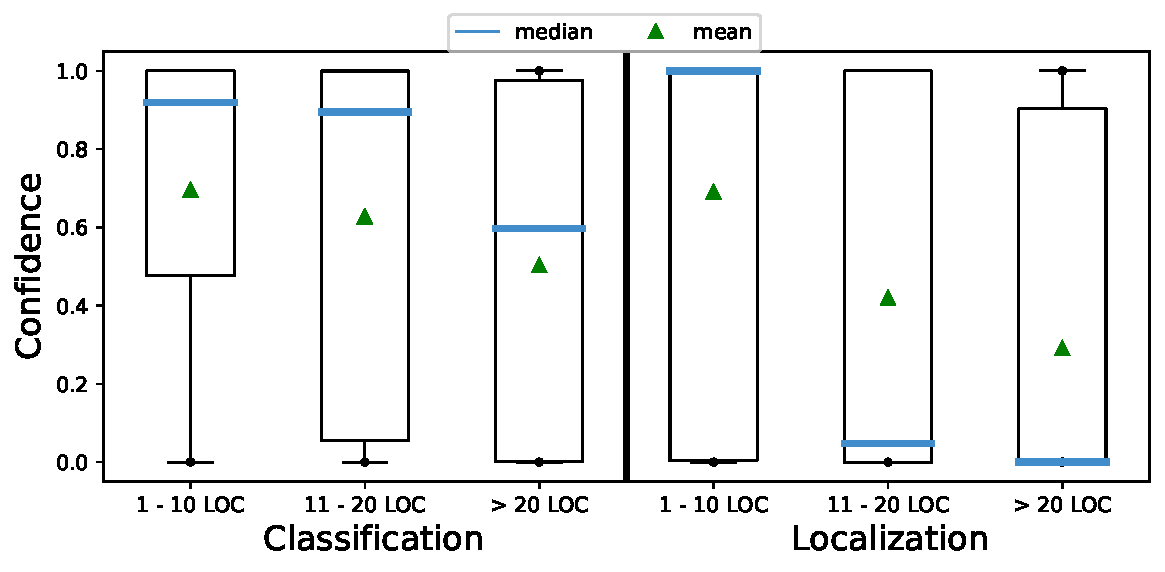
\includegraphics{Fig4b.pdf}
		}
	\end{minipage}
	\caption{Comparison for Fig 4b}
\end{figure*}

 	\begin{figure*}
	\begin{minipage}{0.45\textwidth}
		With retries:
		\centering
		\scalebox{.45}{
			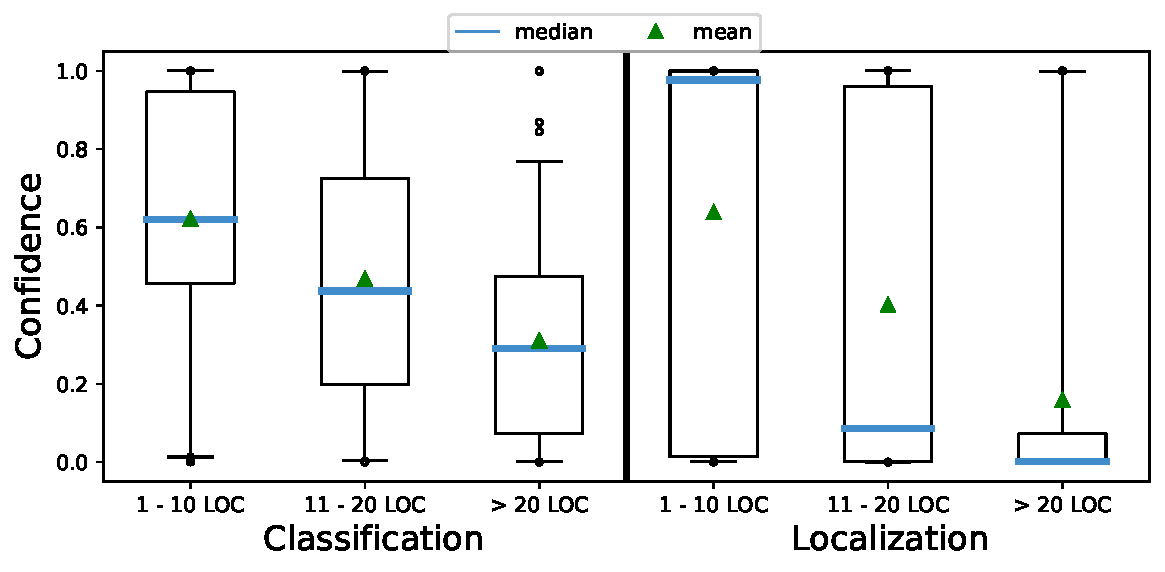
\includegraphics{../Fig4c.pdf}
		}
	\end{minipage}\hfill
	\begin{minipage}{0.45\textwidth}
		Without retries:
		\centering
		\scalebox{.45}{
			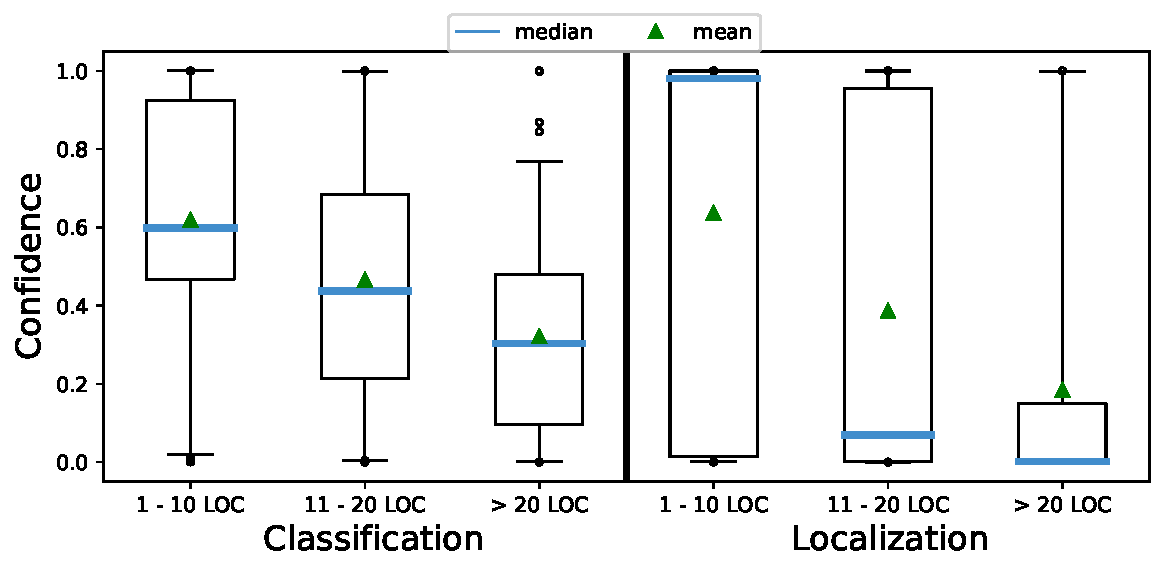
\includegraphics{Fig4c.pdf}
		}
	\end{minipage}
	\caption{Comparison for Fig 4c}
\end{figure*}


 	
 	 	\begin{figure*}
 		\begin{minipage}{0.45\textwidth}
 			With retries:
 			\centering
 			\scalebox{.4}{
 				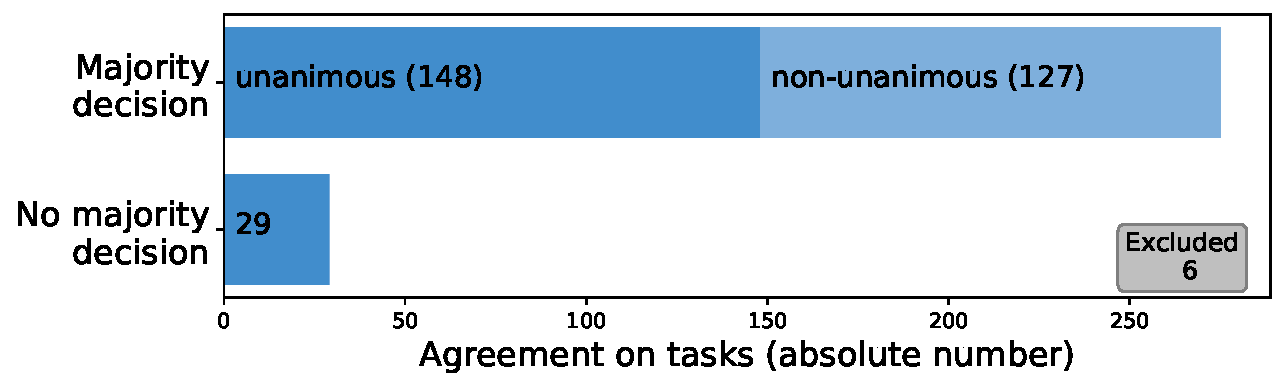
\includegraphics{../Fig5a.pdf}
 			}
 		\end{minipage}\hfill
 		\begin{minipage}{0.45\textwidth}
 			Without retries:
 			\centering
 			\scalebox{.4}{
 				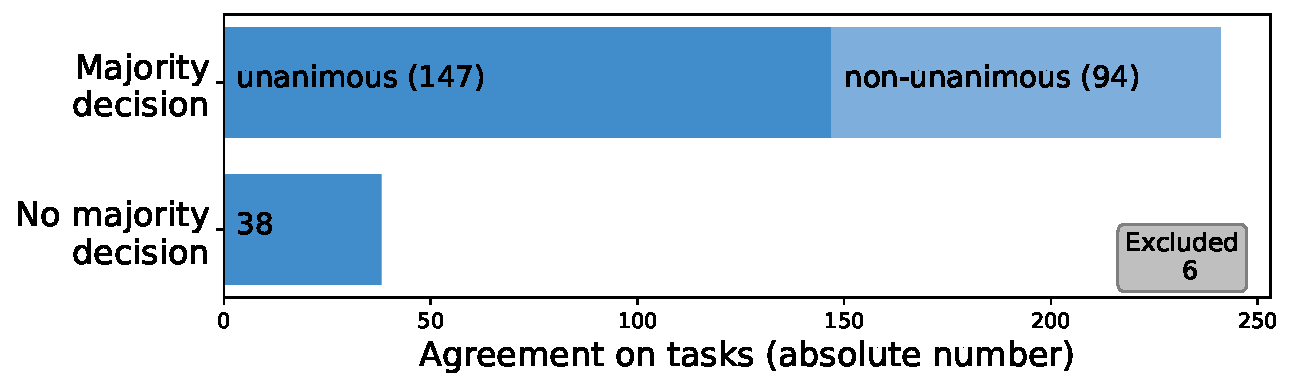
\includegraphics{Fig5a.pdf}
 			}
 		\end{minipage}
 		\caption{Comparison for Fig 5a}
 	\end{figure*}
 	
 	
 	 	 	\begin{figure*}
 		\begin{minipage}{0.45\textwidth}
 			With retries:
 			\centering
 			\scalebox{.4}{
 				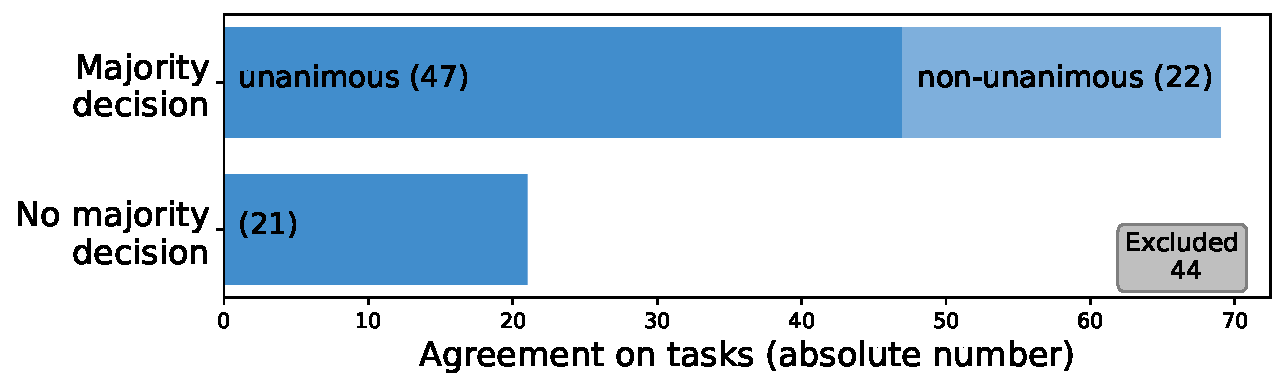
\includegraphics{../Fig5b.pdf}
 			}
 		\end{minipage}\hfill
 		\begin{minipage}{0.45\textwidth}
 			Without retries:
 			\centering
 			\scalebox{.4}{
 				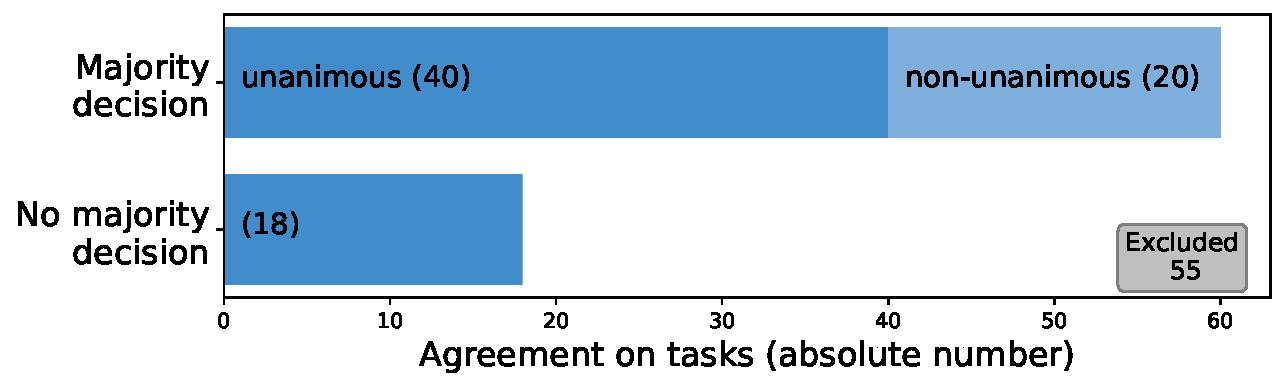
\includegraphics{Fig5b.pdf}
 			}
 		\end{minipage}
 		\caption{Comparison for Fig 5b}
 	\end{figure*}
 
  	 	 	\begin{figure*}
 	\begin{minipage}{0.45\textwidth}
 		With retries:
 		\centering
 		\scalebox{.6}{
 			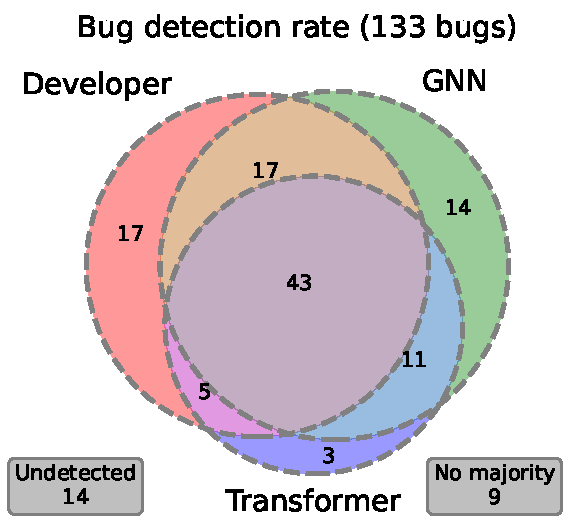
\includegraphics{../Fig6a.pdf}
 		}
 	\end{minipage}\hfill
 	\begin{minipage}{0.45\textwidth}
 		Without retries:
 		\centering
 		\scalebox{.6}{
 			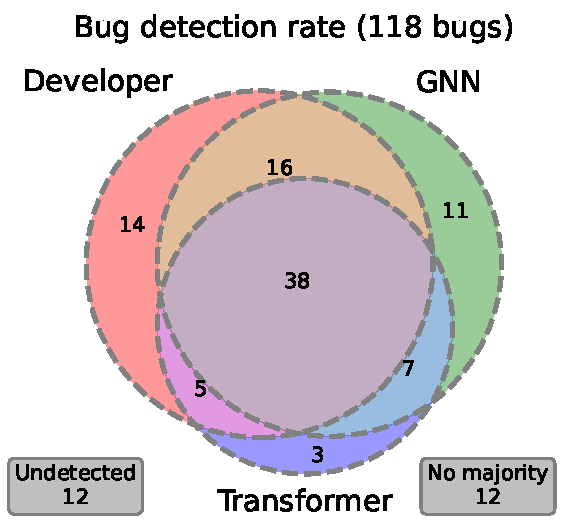
\includegraphics{Fig6a.pdf}
 		}
 	\end{minipage}
 	\caption{Comparison for Fig 6a}
 \end{figure*}

 	 	 	\begin{figure*}
	\begin{minipage}{0.45\textwidth}
		With retries:
		\centering
		\scalebox{.6}{
			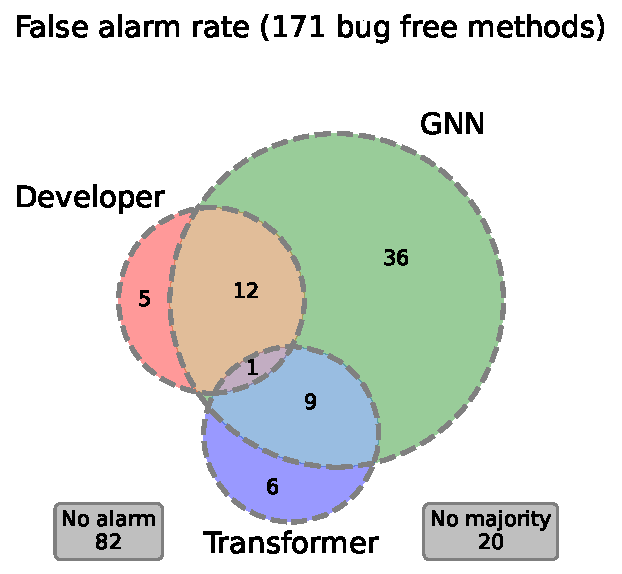
\includegraphics{../Fig6b.pdf}
		}
	\end{minipage}\hfill
	\begin{minipage}{0.45\textwidth}
		Without retries:
		\centering
		\scalebox{.6}{
			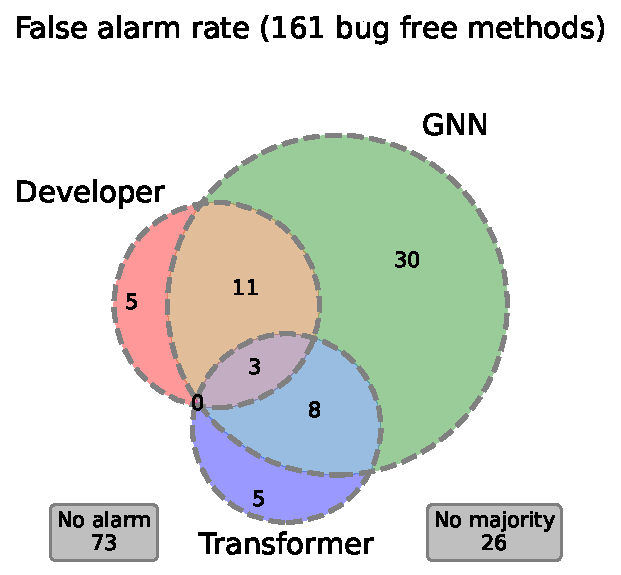
\includegraphics{Fig6b.pdf}
		}
	\end{minipage}
	\caption{Comparison for Fig 6b}
\end{figure*}

 	 	 	\begin{figure*}
	\begin{minipage}{0.45\textwidth}
		With retries:
		\centering
		\scalebox{.6}{
			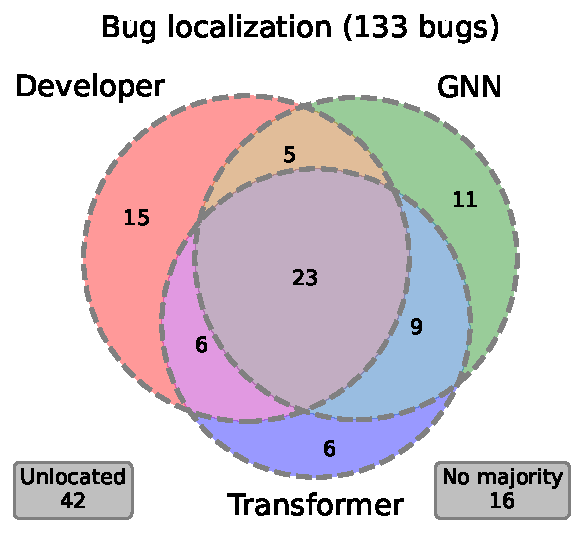
\includegraphics{../Fig6c.pdf}
		}
	\end{minipage}\hfill
	\begin{minipage}{0.45\textwidth}
		Without retries:
		\centering
		\scalebox{.6}{
			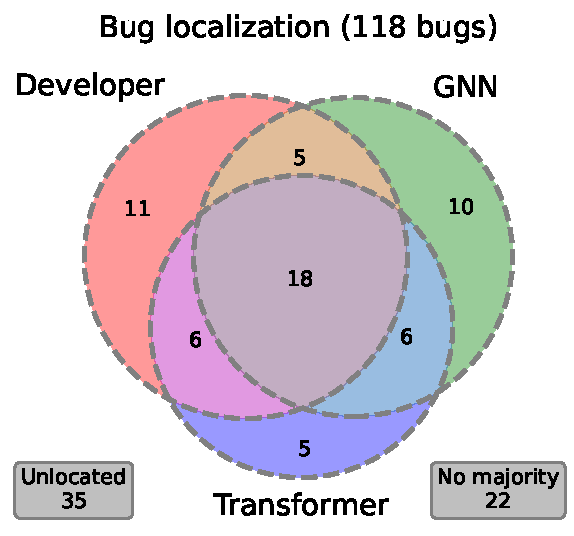
\includegraphics{Fig6c.pdf}
		}
	\end{minipage}
	\caption{Comparison for Fig 6c}
\end{figure*}
 \end{document}